\documentclass[12pt, titlepage]{article}

\usepackage{booktabs}
\usepackage{tabularx}
\usepackage{hyperref}
\usepackage{graphicx}
\hypersetup{
    colorlinks,
    citecolor=blue,
    filecolor=black,
    linkcolor=red,
    urlcolor=blue
}
\usepackage[round]{natbib}

%% Comments

\usepackage{color}

\newif\ifcomments\commentstrue %displays comments
%\newif\ifcomments\commentsfalse %so that comments do not display

\ifcomments
\newcommand{\authornote}[3]{\textcolor{#1}{[#3 ---#2]}}
\newcommand{\todo}[1]{\textcolor{red}{[TODO: #1]}}
\else
\newcommand{\authornote}[3]{}
\newcommand{\todo}[1]{}
\fi

\newcommand{\wss}[1]{\authornote{magenta}{SS}{#1}} 
\newcommand{\plt}[1]{\authornote{cyan}{TPLT}{#1}} %For explanation of the template
\newcommand{\an}[1]{\authornote{cyan}{Author}{#1}}

%% Common Parts

\newcommand{\progname}{Software Engineering} % PUT YOUR PROGRAM NAME HERE
\newcommand{\authname}{Team 21, Visionaries
\\ Ahmed Sahi
\\ Angela Zeng
\\ Ann Shi
\\ Manan Sharma
\\ Stanley Chen} % AUTHOR NAMES                  

\usepackage{hyperref}
    \hypersetup{colorlinks=true, linkcolor=blue, citecolor=blue, filecolor=blue,
                urlcolor=blue, unicode=false}
    \urlstyle{same}
                                


\begin{document}

\title{System Verification and Validation Plan for \progname{}} 
\author{\authname}
\date{\today}
	
\maketitle

\pagenumbering{roman}

\section*{Revision History}

\begin{tabularx}{\textwidth}{p{3cm}p{2cm}X}
\toprule {\bf Date} & {\bf Version} & {\bf Notes}\\
\midrule
2025-10-27 & 1.0 & Add initial draft\\
Date 2 & 1.1 & Notes\\
\bottomrule
\end{tabularx}

~\\

\newpage

\tableofcontents

\newpage

\section{Symbols, Abbreviations, and Acronyms}

\renewcommand{\arraystretch}{1.2}
\begin{tabular}{l p{10cm}} 
  \toprule		
  \textbf{Acronym} & \textbf{Description}\\
  \midrule 
  ET & Eye-tracking: the process of measuring where a person is looking (the gaze point) using specialized hardware, such as wearable glasses.\\
  NTP & Network Time Protocol: used to align timestamps across multiple devices, ensuring synchronized data streams.\\
  CI/CD & Continuous Integration / Continuous Delivery: a software engineering practice involving automated building, testing, and deployment pipelines.\\
  API & Application Programming Interface: defined methods and data formats that allow system components or external applications to communicate.\\
  RBAC & Role-based Access Control: a security model that restricts system access based on user roles and permissions.\\
  POC & Proof-of-Concept: the initial implementation phase (Rev 0) focusing on single-device operation, local data processing, and dashboard visualization.\\
  \bottomrule
\end{tabular}

\newpage

\pagenumbering{arabic}

This document outlines the Verification and Validation (VnV) plan for the group eye-tracking learning platform developed in this capstone project. The purpose of this plan is to establish a structured approach for verifying that the system has been built according to its specifications and validating that it meets its intended purpose.
The plan will detail the methods, tools, and responsibilities involved in increasing the confidence of the developed software. It includes documentation of general information, team roles, verification procedures across the system’s lifecycle stages (requirements, design, and implementation), and both system plus the eventual addition of unit-level test specifications. The document also defines the testing framework for functional and non-functional requirements, along with traceability between requirements, modules, and test cases.



\section{General Information}

\subsection{Summary}

The software being tested is an enhanced version of the \textbf{SocialEyes} framework, a system originally designed for recording and analyzing group gaze data. This project extends the framework to support \textbf{large-group eye-tracking in classroom environments}, implementing both post-session and real-time analytics for instructors to gain insights into their students and teaching.

The system consists of three primary components:

\begin{itemize}
    \item \textbf{Instructor Dashboard with RBAC:} Presents gaze and engagement data in a clear, interpretable format.
    \item \textbf{Post-Session Analytics Module:} Provides aggregated insights to evaluate attention patterns and group interactions after class.
    \item \textbf{Real-Time Analytics Module:} Delivers live feedback to instructors during lectures to support adaptive teaching.
\end{itemize}

Together, these components aim to enhance instructors’ understanding of student engagement and contribute to research on attention and collaboration in learning environments.


\subsection{Objectives}

This project aims to extend the existing SocialEyes system to support real-time session analytics through the integration of a lightweight computer vision algorithm that can efficiently map gaze points from egocentric to central views without compromising accuracy. Verification tests will focus on ensuring that the implemented models will perform correctly and consistently under real-time conditions.
\newline
\newline
Secondary objectives include the creation of the instructor dashboard for visualizing gaze data and providing analytics. Together, these components aim for easy interpretation of gaze-based feedback for instructors to provide useful feedback.
\newline
\newline
Certain objectives will intentionally be excluded due to project constraints. For instance, full verification of the underlying SuperPoint and SuperGlue models and other third-party libraries will not be performed, as these components are assumed to have been previously validated by their original developers. Additionally, large-scale usability testing with diverse participant groups is beyond the project’s current timeframe and resources. 


\subsection{Extras}

This project will include the following extra deliverables that were confirmed during the initial meeting with the project supervisors.

\begin{enumerate}
    \item \textbf{Code Walkthrough Report} \\
    This will be a thorough documentation of the files and folders in the GitHub repository associated with the project.
    
    \item \textbf{User Instruction Video} \\
    This will be an instructional video demonstrating how to interact with the dashboard deliverable of the project for each of the user roles (e.g., instructor).
\end{enumerate}


\subsection{Relevant Documentation}

The Verification and Validation (V\&V) Plan is dependent on and supported by several key project documents that define the foundation, scope, and success criteria for the group eye-tracking learning platform. These documents collectively guide how requirements are verified and validated throughout the development process.
\newline
\newline
\textbf{Software Requirements Specification (SRS)}
\newline
The \textit{Software Requirements Specification (SRS)} defines the functional and non-functional requirements of the system, serving as the primary reference for the verification process. It specifies what the system must do, how it should perform, and the constraints under which it must operate. Each verification test will be mapped to one or more requirements defined in the SRS.
\newline
\newline
\textbf{Development Plan}
\newline
The \textit{Development Plan} outlines the project’s implementation roadmap, including project decomposition, proof-of-concept demonstrations, and the technologies used to conduct it. It informs the scheduling and prioritization of verification and validation activities, ensuring that testing aligns with the overall development timeline and that each module is verified at appropriate stages in the lifecycle.
\newline
\newline
\textbf{Problem Statement and Goals Document}
\newline
The \textit{Problem Statement and Goals Document} defines the motivation, context, and intended impact of the project. It provides the conceptual foundation for validation activities, ensuring that the developed system not only meets its technical specifications but also fulfills its educational and research goals. This document reinforces the relevance of the V\&V Plan by providing a basis for why the tests being verified are crucial for achieving the project’s goals.
\newline
\newline

\section{Plan}

\subsection{Verification and Validation Team}

The Verification and Validation process for this project will involve both the planning and testing teams, as well as the project supervisor and members of the research group.\\

\textbf{Planning team:} Stanley Chen, Ann Shi, and Ibrahim Sahi will be responsible for developing review plans for SRS, VnV, and other documentation, as well as plans for design, implementation and software verification.\\

\textbf{Testing team:} Manan Sharma and Angela Zang will focus on developing and executing system tests that confirm the implementation satisfies the functional and non-functional requirements defined in the SRS.\\

The supervisor and research collaborators will provide support through reviewing and validating the planned systems.

\subsection{SRS Verification}

To ensure that the Software Requirements Specification is accurate, comprehensive, and aligned with the project’s goals, a two-stage review process will be used: a preliminary peer review followed by a structured team review meeting.\\

\textbf{Peer Review}\\

An initial peer review will be conducted by classmates to identify issues in readability, organization, and completeness. This step helps ensure that the SRS communicates effectively to a general audience and that the flow, terminology, and formatting are clear.\\

\textbf{Research Team Review Meeting}\\

A review meeting will be held with the research team during the routine meeting time. This session will combine the technical, instructional, and managerial perspectives required to validate the SRS in a single coordinated effort. During the meeting, a condensed version of the SRS will be presented, highlighting key sections such as system scope, functional and non-functional requirements, datasets, technology dependencies and goals. The review will be guided using a task-based inspection, structured around each participant’s perspective.\\

Instructors will verify that the system goals, use cases, and requirements align well with their needs as the primary users. Researchers will assess the logical soundness of the proposed workflows and ensure that data collection and analysis described in the SRS are technically consistent. The Supervisor will evaluate the overall feasibility of the system, ensuring that the listed technologies, environments, and resources are accessible and that the project remains within defined scope and constraints.\\

Feedback will be collected in real time and logged into the project’s issue tracker for traceability.\\


\subsection{Design Verification}

To ensure that the system design aligns with the functional and non-functional requirements described in the SRS, the team will conduct a structured design review process composed of three complementary activities.\\

First, internal peer review sessions will be held to inspect the Modular Interface Specification (MIS) and system architecture diagrams using a prepared checklist. The checklist will focus on completeness, traceability, modularity, and adherence to design principles such as separation of concerns and single responsibility. Each module (for example, the data ingestion service, analytics engine, and instructor dashboard) will be verified to ensure its interface definitions are consistent with its described purpose and expected data flows.\\

Second, a cross-team review will be conducted with another capstone team to identify design ambiguities and potential integration issues from an external perspective. Feedback from this review will be recorded in the GitHub issue tracker for traceability.\\

Finally, the design documents, including component diagrams and data-flow models, will be presented to the project supervisors for validation of research-specific considerations such as synchronization accuracy between multiple gaze streams and the interpretability of dashboard metrics.\\

Identified defects or improvement items will be categorized as documentation, logic, or scope issues, prioritized, and resolved before implementation. Evidence of completion will be stored as annotated PDFs and issue links within the project repository.\\

\subsection{Verification and Validation Plan Verification}

The verification and validation plan will also undergo verification to ensure that it is internally consistent, complete, and feasible given the project timeline. This will be achieved through a combination of peer inspection, supervisor validation, and cross-artifact consistency checks.\\

Classmates will conduct a checklist-based inspection to evaluate the clarity of objectives, completeness of planned tests, and consistency of terminology with the SRS. The supervisors will review the document to confirm that the chosen verification and validation techniques, such as unit testing, usability testing, and performance evaluation, are appropriate for both the engineering and research goals of the project.\\

In addition, the VnV Plan will be cross-checked against the Development Plan and Hazard Analysis documents to ensure that testing activities address identified risks such as privacy concerns or latency issues. Any inconsistencies found will be logged in the issue tracker under the label \texttt{type:docs} and corrected before the next revision. This approach ensures that the VnV Plan remains an up-to-date reflection of the team’s testing progress.\\

\subsection{Implementation Verification}

Implementation verification ensures that the developed system conforms to the verified design and meets the requirements specified in the SRS. Verification will be performed through a combination of automated and manual activities.\\

Automated unit and integration tests will be created for each module of the system, including the backend API, real-time analytics processor, and React dashboard. These will be implemented using PyTest for Python and Jest for JavaScript. Test coverage percentage and pass/fail status will be tracked through GitHub Actions to maintain continuous integration.\\

Static analysis and linting will be performed using ESLint, Prettier, and flake8 to enforce coding standards and detect syntax or style violations. Before Revision 0, the team will conduct a supervised code walkthrough with the project supervisor, where each developer will explain their module’s implementation and trace its connection to the system requirements.\\

Each new feature merged into the main branch will automatically trigger a CI/CD pipeline that runs all tests to prevent regressions. In addition, static verification of documentation will be performed to detect outdated comments or broken references between source code and documentation.\\

\subsection{Automated Testing and Verification Tools}

Automation is a central part of the verification strategy, ensuring that every commit is tested consistently. The following tools and frameworks will be used throughout development.\\

\begin{table}[htbp]
\centering
\caption{Automated Testing and Verification Tools}
\begin{tabularx}{\textwidth}{|p{3cm}|p{4cm}|X|}
\hline
\textbf{Tool} & \textbf{Purpose} & \textbf{Verification Activity} \\
\hline
GitHub Actions & Continuous integration pipeline that runs automatically on each pull request & Executes all test suites, linting, and build checks. Prevents merges if tests fail. \\
\hline
PyTest & Python testing framework for backend and data processing modules & Unit tests for data parsing, computation accuracy, and real-time gaze mapping \\
\hline
Jest and React Testing Library & Front-end testing for user interface components and data visualizations & Verifies correct rendering and state management on the instructor dashboard \\
\hline
ESLint, Prettier, and flake8 & Static code analysis and style enforcement tools & Ensures consistent syntax, formatting, and code quality \\
\hline
Valgrind or cProfile & Profiling and memory analysis tools & Identifies performance bottlenecks and inefficiencies in real-time data handling \\
\hline
Coverage.py and Codecov & Code coverage tracking utilities & Measures test completeness and identifies untested portions of the codebase \\
\hline
Docker & Reproducible environment for testing and deployment & Verifies installability and portability of the full system across different machines \\
\hline
\end{tabularx}
\end{table}

At the end of each development iteration, the CI dashboard will export a summary of test coverage, lint violations, and failed cases. These results will be included in the final VnV Report as objective evidence of verification and overall system reliability.\\

\subsection{Software Validation}

The validation of the enhanced SocialEyes framework will primarily be conducted through regular review sessions and iterative demonstrations with project supervisors Dr. Lauren Fink and Dr. Irene Yuan. Weekly meetings will serve as checkpoints to assess progress against the requirements outlined in the Software Requirements Specification (SRS), ensuring that the evolving system aligns with both the technical and research goals of the project.
\newline
A formal Rev 0 demonstration will be presented to the supervisors once completed. This demo will be used to validate that the core system features—real-time gaze analytics, post-session data visualization, and the instructor dashboard—accurately reflect the intended requirements and provide value within a classroom context. Feedback from this session will guide subsequent iterations and refinement of the system.
In addition to supervisor reviews, user validation will be obtained through feedback from a postdoctoral researcher affiliated with the SocialEyes project who has experience conducting lectures and an interest in applying this technology to teaching contexts. This will help validate the system’s usability and relevance from an instructor’s perspective.
\newline

\section{System Tests}

\subsection{Tests for Functional Requirements}

This subsection provides concrete, executable tests for all Functional Requirements (FRs) in the SRS.
Tests are grouped by subsystem: Data Acquisition and Ingestion; Data Processing and Analytics; Data
Management and Backend Services; Visualization and Dashboard Interface; and Supporting Infrastructure
(and Stretch). Each test specifies Control, Initial State, Input, Output (expected result), Test Case
Derivation, Test Data / Artefacts, and How the test will be performed.

\subsubsection{Area of Testing 1 - Data Acquisition and Ingestion}

Note: This area covers FR-1, FR-2, FR-3, FR-5, FR-6, and FR-19 from the SRS (operational modes, instructor session control, device capture, synchronization, recovery, and pre-session calibration).

\paragraph{Mode Switching and Session Control}

\begin{enumerate}

\item \textbf{FR-1-T1} \\

Control: Automatic

Initial State: System services running; no active session; device simulator available.

Input: (1) From dashboard, start a Recording session and run for 10 s. (2) Switch to Streaming mode via a UI toggle while the session is active.

Output: Session state transitions succeed; no crash; data continuity preserved with no inter-packet gap greater than 100 ms around the switch.

Test Case Derivation: FR-1 requires support for Recording and Streaming operational modes to enable both offline analysis and real-time visualization.

\textit{Test Data / Artefacts:} Synthetic gaze stream (JSON/Parquet), egoview video (MP4/MKV), session state logs (LOG/CSV).

How test will be performed: A UI test script triggers the state changes. A log parser computes inter-packet gaps from ingest timestamps and asserts the maximum gap is less than or equal to 100 ms.

\item \textbf{FR-2-T1 - Instructor Session Controls (Start/Pause/Resume/Stop)} \\

Control: Manual + Automatic

Initial State: Instructor role authenticated; dashboard open on Sessions page.

Input: Click Start, then Pause after 5 s, then Resume after 5 s, then Stop.

Output: UI status changes Active $\rightarrow$ Paused $\rightarrow$ Active $\rightarrow$ Stopped. No data are stored during the pause interval.

Test Case Derivation: FR-2 mandates instructor control to ensure intentional and ethical recording.

\textit{Test Data / Artefacts:} Test user accounts (CSV/YAML), RBAC policy (YAML), session metadata export (CSV), event logs (LOG).

How test will be performed: Tester performs the sequence in the UI while a script queries session metadata and verifies there are no gaze or frame records timestamped within the pause window.

\item \textbf{FR-3-T1 - Device Data Acquisition via External API} \\

Control: Integration (Automatic)

Initial State: Eye-tracking device or simulator connected and reachable via API.

Input: Issue Start Recording.

Output: Synchronized gaze samples and egoview frames are received at expected rates and timestamped.

Test Case Derivation: FR-3 specifies interfacing with supported eye-tracking devices to collect synchronized gaze and video.

\textit{Test Data / Artefacts:} Device API mock responses (JSON), captured video (MP4/MKV), gaze samples (JSON/Parquet), device/config settings (YAML).

How test will be performed: An integration test hits the device API simulator, records 30 s, and checks that sample and frame counts and timestamps are within expected tolerances.

\item \textbf{FR-5-T1 - Multi-Device Time Synchronization} \\

Control: Automatic

Initial State: Two device simulators streaming; NTP service active.

Input: Emit a visible synchronization cue at time t0.

Output: Detected cue timestamps differ by no more than 20 ms across the two devices.

Test Case Derivation: FR-5 requires time-aligned data streams for valid group analysis.

\textit{Test Data / Artefacts:} Dual-stream video with sync cue (MP4), NTP/sync logs (LOG), cue-detection script output (CSV).

How test will be performed: A detector finds the cue frame in both streams and compares timestamps after offset correction.

\item \textbf{FR-6-T1 - Recovery After Transient Network Loss} \\

Control: Automatic

Initial State: Active streaming session (video and gaze).

Input: Introduce a 2 s network drop and then restore the link.

Output: Stream resumes within 5 s of link restoration; the session remains a single continuous session.

Test Case Derivation: FR-6 requires resumption within 5 s for short connectivity issues.

\textit{Test Data / Artefacts:} Network shaping profile (SH/TC config), ingest/application logs (LOG), optional packet capture (PCAP), timing summary (CSV).

How test will be performed: A traffic shaper introduces the drop. The harness measures restoration and resume times and asserts resume within 5 s.

\item \textbf{FR-19-T1 - Automatic Calibration Check Before Recording} \\

Control: Automatic

Initial State: Device connected; no active session.

Input: Click Start Recording.

Output: If calibration score is below threshold, recording is blocked and the user is prompted to recalibrate. If the score meets threshold, recording starts and a CalibrationPassed event is logged.

Test Case Derivation: FR-19 prevents poor data due to miscalibration.

\textit{Test Data / Artefacts:} Calibration result payloads (JSON), UI evidence (PNG screenshot), calibration/decision logs (LOG).

How test will be performed: Mock the device API to return failing and passing calibration states; verify gating and log entries.

\end{enumerate}


\subsubsection{Area of Testing 2 - Data Processing and Analytics}

Note: This area covers FR-7, FR-8, FR-9, FR-10, FR-20, and FR-24 from the SRS (filtering and correction, projection to a shared space, real-time metrics, post-session analytics, off-screen filtering, and replay).

\paragraph{Analytics Correctness and Latency}

\begin{enumerate}

\item \textbf{FR-7-T1 - Noise and Blink Filtering} \\

Control: Automatic

Initial State: Offline dataset with labeled blink and noise segments.

Input: Run processing pipeline on the dataset.

Output: At least 95\% of labeled blink/noise samples are removed and no more than 2\% of valid samples are removed incorrectly.

Test Case Derivation: FR-7 requires filtering and correction to ensure reliable metrics.

\textit{Test Data / Artefacts:} Labeled blink/noise dataset (CSV), raw gaze stream (Parquet/CSV), filter pipeline configuration (YAML), accuracy report (CSV).

How test will be performed: Compare algorithm output masks to labels; compute precision and recall; assert thresholds.

\item \textbf{FR-8-T1 - Gaze Projection to Shared Coordinate Space} \\

Control: Automatic

Initial State: Egoview frames and central-view frames with visible fiducial markers.

Input: Run the projection to map egocentric gaze to central coordinates.

Output: Mean projection error is less than 3\% of the central-view width; 95th percentile error is less than 10\%.

Test Case Derivation: FR-8 requires accurate projection for group alignment.

\textit{Test Data / Artefacts:} Egoview frames (PNG/JPG), central-view frames (PNG), fiducial/scene map (JSON), projected gaze coordinates (CSV).

How test will be performed: Compute 2D error against fiducial ground truth and assert thresholds.

\item \textbf{FR-9-T1 - Real-Time Metric Latency} \\

Control: Automatic

Initial State: Live stream active; dashboard metrics panel visible.

Input: Stream a scripted gaze trajectory for 60 s.

Output: Metric widgets (velocity, entropy, normalized contour area) update with end-to-end delay less than or equal to 1 s and an effective refresh rate near 20 Hz.

Test Case Derivation: FR-9 specifies real-time computation to support instructional feedback.

\textit{Test Data / Artefacts:} Synthetic trajectory specification (JSON), backend metric logs (LOG), frontend render timestamps (CSV), browser/version note (TXT).

How test will be performed: Backend stamps metric times; frontend logs render times; a script computes latency and effective rate.

\item \textbf{FR-20-T1 - Off-Screen and Invalid Gaze Exclusion} \\

Control: Automatic

Initial State: Dataset with labeled off-screen intervals.

Input: Run real-time and post-session analysis modules.

Output: At least 98\% of off-screen points are flagged and excluded from aggregates; no flagged points appear in heatmaps.

Test Case Derivation: FR-20 requires excluding invalid gaze to prevent misinterpretation.

\textit{Test Data / Artefacts:} Off-screen ground-truth labels (CSV), raw gaze stream (Parquet/CSV), exclusion flags (CSV), generated heatmap (PNG).

How test will be performed: Compute confusion matrix against labels; verify heatmap generator omits flagged points.

\item \textbf{FR-10-T1 - Post-Session Summary Generation} \\

Control: Automatic

Initial State: One completed recording with known scripted attention shifts.

Input: Invoke Generate Summary.

Output: Exported CSV, JSON, and PNG include: session heatmap, time-series of engagement, and participant-level statistics that match an independently recomputed reference within plus or minus 2\%.

Test Case Derivation: FR-10 requires generation of post-session analytics.

\textit{Test Data / Artefacts:} Completed session data (CSV/Parquet), system exports (CSV/JSON/PNG), independent recomputation outputs (CSV/JSON).

How test will be performed: An independent script recomputes metrics from raw data; differences are compared and asserted.

\item \textbf{FR-24-T1 - Replay and Re-Analysis Consistency} \\

Control: Manual + Automatic

Initial State: Stored session available in the replay view.

Input: Play the session from start to finish and trigger Re-run Analytics.

Output: Event timing during replay matches original within less than 50 ms; recomputed metrics differ by less than 1\% from the original.

Test Case Derivation: FR-24 enables verification and debugging using replay.

\textit{Test Data / Artefacts:} Replay media (MP4/MKV), original metric series (CSV), recomputed metric series (CSV), event markers (CSV).

How test will be performed: Compare timestamped events and metric series to the original outputs; assert thresholds.

\end{enumerate}


\subsubsection{Area of Testing 3 - Data Management and Backend Services}

Note: This area covers FR-11, FR-12, FR-13, FR-22, and FR-23 from the SRS (persistence, metadata, APIs, traceability, and configurability).

\paragraph{Persistence, Metadata, APIs, and Configurability}

\begin{enumerate}

\item \textbf{FR-11-T1 - Data Persistence Across Restarts} \\

Control: Automatic

Initial State: Clean database; services running.

Input: Record 2 minutes; stop; restart services; load the session.

Output: Raw frames, gaze samples, and derived analytics are present and readable after restart.

Test Case Derivation: FR-11 requires local storage of raw and processed data.

\textit{Test Data / Artefacts:} Database schema (SQL), database snapshot (SQL dump), session directory (mixed files as produced).

How test will be performed: An integration script records, restarts the stack, and then queries by session ID to validate counts and checksums.

\item \textbf{FR-12-T1 - Session Metadata Completeness} \\

Control: Automatic

Initial State: None.

Input: Start and stop a session with two participants.

Output: The session record contains timestamp, session ID, and participant IDs; each data row references the session ID.

Test Case Derivation: FR-12 mandates metadata for traceability.

\textit{Test Data / Artefacts:} Session and participant schemas (DDL/CSV), example record export (CSV), integrity check script (SQL).

How test will be performed: SQL assertions check required columns and foreign key presence.

\item \textbf{FR-13-T1 - Programmatic API for Analytics Retrieval} \\

Control: Automatic

Initial State: One completed session with analytics.

Input: GET /api/sessions/\{id\}/analytics and POST /api/session/start.

Output: HTTP 200 with schema-valid JSON for analytics; start endpoint returns a new session ID.

Test Case Derivation: FR-13 requires APIs for analytics retrieval and session management.

\textit{Test Data / Artefacts:} API specification (OpenAPI YAML), API test collection (JSON), example analytics response (JSON).

How test will be performed: An automated API test validates response codes and JSON schema.

\item \textbf{FR-22-T1 - Traceability From Raw to Reports} \\

Control: Automatic

Initial State: Completed session.

Input: Trace query joining raw, processed, and report tables on session ID.

Output: Complete lineage from raw to processed to export; no orphan rows.

Test Case Derivation: FR-22 requires maintained traceability via unique session identifiers.

\textit{Test Data / Artefacts:} Traceability query (SQL), table extracts for raw/processed/reports (CSV), lineage visualization (PNG/PDF).

How test will be performed: SQL join plus referential integrity checks; fail on nulls or orphans.

\item \textbf{FR-23-T1 - Configuration Changes Take Effect} \\

Control: Automatic

Initial State: Default configuration applied.

Input: Change data directory, export format, and device ID in configuration; restart.

Output: Next session writes to the new directory; exports match the configured formats; device routing uses the new ID.

Test Case Derivation: FR-23 enables flexible deployment without code changes.

\textit{Test Data / Artefacts:} Configuration file (YAML/TOML), directory listings (TXT), export manifest (JSON).

How test will be performed: Start a session and verify filesystem paths, export set, and device mapping.

\end{enumerate}


\subsubsection{Area of Testing 4 - Visualization and Dashboard Interface}

Note: This area covers FR-14, FR-15, FR-16, FR-26, and FR-27 from the SRS (RBAC, real-time visual analytics, exports, status indicators, and spatial masking/anonymization).

\paragraph{Access, Status, Exports, and Privacy}

\begin{enumerate}

\item \textbf{FR-14-T1 - Role-Based Access Control} \\

Control: Automatic

Initial State: Two users exist: instructor and unauthorized.

Input: Both users attempt to access Live Analytics and Export views.

Output: Instructor gains access; unauthorized user receives 403 Forbidden; no data leakage occurs.

Test Case Derivation: FR-14 enforces authentication and authorization for sensitive data.

\textit{Test Data / Artefacts:} Test user list (CSV), RBAC policy (YAML), audit log (LOG), denied-access summary (CSV).

How test will be performed: API and UI tests simulate both roles; backend audit logs are checked for denied attempts.

\item \textbf{FR-15-T1 - Real-Time Visual Analytics Render} \\

Control: Automatic

Initial State: Live stream; dashboard analytics tab open.

Input: 60 s of synthetic gaze with known hotspots.

Output: Heatmap tiles and engagement widgets update within 1 s after data arrival and reflect hotspots in the correct regions.

Test Case Derivation: FR-15 requires real-time visual analytics on the dashboard.

\textit{Test Data / Artefacts:} Synthetic hotspot definition (JSON), UI render timestamps (CSV), reference heatmap (PNG).

How test will be performed: DOM probes read widget timestamps; a reference heatmap is computed independently and compared with the rendered result.

\item \textbf{FR-16-T1 - Export Formats and Fidelity} \\

Control: Manual + Automatic

Initial State: Completed session with analytics.

Input: User exports CSV, JSON, and PNG.

Output: Files exist; CSV and JSON schemas are valid; the PNG heatmap visually matches the dashboard with structural similarity index greater than 0.95.

Test Case Derivation: FR-16 requires export of post-session analytics in common formats.

\textit{Test Data / Artefacts:} CSV schema (CSV schema file), JSON schema (JSON schema file), exported outputs (CSV/JSON/PNG), dashboard render reference (PNG).

How test will be performed: A schema validator checks CSV and JSON; an SSIM comparison is run on the PNG versus a server-side render.

\item \textbf{FR-26-T1 - Status Indicators (Latency, Jitter, Drift)} \\

Control: Automatic

Initial State: Live session; status panel visible.

Input: Inject synthetic 150 ms network jitter and 10\% packet loss for 20 s.

Output: Indicators reflect increased latency and loss within two refresh cycles; synchronization drift increases accordingly.

Test Case Derivation: FR-26 requires real-time system status indicators.

\textit{Test Data / Artefacts:} Network impairment profile (SH/TC config), status endpoint samples (JSON), metrics time-series (CSV).

How test will be performed: Traffic shaping is applied; displayed metrics are sampled via test hooks and compared to injected conditions.

\item \textbf{FR-27-T1 - Spatial Masking and Anonymization} \\

Control: Manual + Automatic

Initial State: Privacy mask polygon configured to exclude a region.

Input: Record 30 s with participants present in the masked area; export heatmap and a representative frame.

Output: No identifiable faces or eyes appear in the masked region; exported data for masked pixels are absent or blurred.

Test Case Derivation: FR-27 requires definable exclusion zones for privacy in storage and export.

\textit{Test Data / Artefacts:} Mask configuration (JSON), exported frame (PNG), heatmap (PNG), face-detector output (CSV).

How test will be performed: An automated face detector confirms zero detections inside the mask; a manual spot-check verifies exports.

\end{enumerate}


\subsubsection{Area of Testing 5 - Supporting Infrastructure and Stretch (Optional)}

Note: This area covers FR-18 (logging/monitoring) and Stretch FR-4, FR-17, FR-21, FR-25 (Rev 1+ goals).

\paragraph{Observability, Roles, Privacy Pipeline, and Scalability}

\begin{enumerate}

\item \textbf{FR-18-T1 - Runtime Logging and Metrics} \\

Control: Automatic

Initial State: Logging level = INFO; metrics collector enabled.

Input: Run a 2 min session with one induced warning (device reconnect).

Output: Log contains timestamped events for start/stop, warnings, and metrics snapshots; metrics series include FPS, jitter, and dropped frames.

Test Case Derivation: FR-18 requires logging diagnostics and performance metrics for monitoring.

\textit{Test Data / Artefacts:} Logging configuration (YAML), runtime logs (LOG), metrics export (CSV), event list (CSV).

How test will be performed: Parse logs and metrics endpoint; assert presence and cadence.

\item \textbf{FR-4-T1 - Central Camera Integration (Stretch)} \\

Control: Integration (Automatic)

Initial State: Central-camera RTSP source available.

Input: Start session with central-view enabled; two egoviews active.

Output: Central view frames are timestamped and aligned with egoviews; the projection module accepts the central feed without error.

Test Case Derivation: FR-4 optionally interfaces with a central camera for shared-scene alignment.

\textit{Test Data / Artefacts:} RTSP stream configuration (TXT), central-view video (MP4), alignment results (CSV), error logs (LOG).

How test will be performed: RTSP ingest with timestamp alignment check; verify projection module operates with the central frames present.

\item \textbf{FR-17-T1 - Role-Based View Separation (Stretch)} \\

Control: Manual + Automatic

Initial State: Two roles exist: Instructor and Researcher.

Input: Log in as each role and open the dashboard.

Output: Instructor view hides researcher-only analytics (and vice versa); access attempts outside role return 403 Forbidden.

Test Case Derivation: FR-17 provides separate role-based views to enhance usability and compliance.

\textit{Test Data / Artefacts:} Role/view configuration (YAML), UI screenshots (PNG), endpoint access matrix (CSV), audit logs (LOG).

How test will be performed: UI inspection combined with API role assertions and audit log checks.

\item \textbf{FR-21-T1 - Privacy Anonymization Pipeline (Stretch)} \\

Control: Manual + Automatic

Initial State: Example frames containing identifiable faces and eyes; anonymization enabled.

Input: Export video frame and heatmap with anonymization on.

Output: No identifiable faces or eye images remain; face detector confidence below threshold throughout; heatmap contains no pixel data from masked regions.

Test Case Derivation: FR-21 ensures ethical compliance and participant anonymity in exports.

\textit{Test Data / Artefacts:} Example frames for anonymization (PNG), anonymized outputs (PNG), detector results (CSV), privacy compliance checklist (PDF/MD).

How test will be performed: Automated face-blur verification plus manual review of a sample of exports.

\item \textbf{FR-25-T1 - Multi-Device Scaling (Stretch)} \\

Control: Automatic

Initial State: Ten device simulators configured.

Input: Start streaming all 10 concurrently for 5 min.

Output: Inter-device synchronization drift stays within $\pm 20$ ms; no ingest backpressure beyond configured queue thresholds; no service crash.

Test Case Derivation: FR-25 targets scaling to $\ge 10$ devices while maintaining synchronization accuracy.

\textit{Test Data / Artefacts:} Multi-device simulator configuration (YAML), system metrics (CSV), synchronization drift summary (CSV), queue depth logs (CSV).

How test will be performed: Synthetic load plus synchronization measurement as in FR-5-T1; report drift statistics and queue depths.

\end{enumerate}


\subsection{Tests for Nonfunctional Requirements}

\begin{enumerate}

\subsubsection{Performance, Reliability, and Scalability Tests}

\item{TC-NFR-1-Latency\\} 
Type: Dynamic, Automated\\ 

Initial State: Both backend and frontend are running locally and the system is connected to mock eye tracking data source.\\

Input/Condition: Conduct a 30 min, test session with simulated eye tracking and video data. Then record the timestamps of when data is recorded, processed and displayed.\\ 

Output/Result: Record the average latency between capturing and visualizing data. Pass if latency is less than 1.5 s.\\ 

How test will be performed: Log the timestamp when data is inputted, and when the dashboard is updated. Then compute the delay from the logs of timestamps.\\ 

\item{TC-NFR-2-UpdateHz\\} 
Type: Dynamic, Automated\\ 

Initial State: Dashboard is rendering heatmaps in browser.\\ 

Input/Condition: For a 10 min session, with browser performance logs recording the render times.\\ 

Output/Result: Average and 95th percentile render frequency. Test will pass if the mean is greater than 20 Hz and the 95th percentile is greater than 18 Hz. This will include FPS histogram and timeline graph.\\ 

How test will be performed: The performance at each render will be recorded by using a Javascript probe, then the data will be summarized automatically in the command line.\\ 

\item{TC-NFR-3-SyncDrift\\}
Type: Dynamic, Automated\\

Initial State: 3 to 10 devices synchronized via Network Time Protocol (NTP), all streaming gaze and egoview data under standard classroom conditions.\\

Input/Condition: Each device emits synchronization markers once per second during a session.\\

Output/Result: Time-difference series between devices with maximum drift per minute recorded. Pass if drift stays within 20 ms.\\

How test will be performed: Match sync markers by frame index across devices and compute drift statistics to verify requirement.

\item{TC-NFR-4-JitterLoss\\}
Type: Dynamic, Automated\\

Initial State: Live data streaming between devices and analytics backend.\\

Input/Condition: Browser script sends WebSocket heartbeat every 100 ms while measuring round-trip delay.\\

Output/Result: Logs containing average, P95, and maximum jitter and a chart of packet loss vs jitter.\\

How test will be performed: Browser records timestamps for sent/received messages, computes latency variation, and summarizes results in dashboard or CI logs.

\item{TC-NFR-16-Scale10\\}
Type: Load\\

Initial State: Backend services running, synthetic gaze stream generators configured.\\

Input/Condition: Simulate 1, 3, 5, and 10 devices concurrently for up to 20 minutes each, streaming gaze data at normal rates.\\

Output/Result: CPU and memory usage, latency percentiles, and sync error recorded. Pass if sync error < 20 ms at 10 devices. Produce plots of latency vs device count and sync error vs device count.\\

How test will be performed: Use synthetic streams to simulate multiple devices while collecting system metrics; visualize results.

\item{TC-NFR-5-AutoRecover\\}
Type: Dynamic, Automated\\

Initial State: Multiple devices actively streaming gaze data to backend.\\

Input/Condition: Intentionally disconnect each device stream for 10 seconds at randomized intervals, repeated 20 times.\\

Output/Result: Reconnection time for each disconnection; pass if all streams automatically reconnect without data loss or corruption.\\

How test will be performed: Scripted disconnections; backend verifies reconnection by checking frame sequence continuity and comparing checksums before/after reconnection.

\item{TC-NFR-6-Uptime\\}
Type: Long-run observation\\

Initial State: Full classroom analytics system deployed and running under normal conditions.\\

Input/Condition: Conduct three scheduled 90-minute sessions across one week while tracking uptime metrics.\\

Output/Result: Summary report with total uptime percentage, number of downtime incidents, and average recovery time.\\

How test will be performed: Send a signal every 10 seconds; missed signals logged as downtime and recovery duration measured.

\item{TC-NFR-17-TimeACID\\}
Type: Dynamic, Static\\

Initial State: Database running and handling necessary operations.\\

Input/Condition: Insert 10,000 events with known timestamps while performing multiple transactions.\\

Output/Result: Timestamp drift within 33 ms and ACID properties maintained.\\

How test will be performed: Compare database timestamps to ingestion clock and verify transactions commit/rollback correctly using transactional test suite.

\item{TC-NFR-18-BigSession\\}
Type: Load test\\

Initial State: System ready for large-scale data intake.\\

Input/Condition: Process 50 x 200 GB of generated session data while running ingestion and analytics queries concurrently.\\

Output/Result: Throughput and query latency remain stable; record any performance degradation or curves.\\

How test will be performed: Batch load generated data, monitor CPU/memory (Prometheus), and measure query response times under increasing load.

\item{TC-NFR-26-BackupRestore\\}
Type: Static, Dynamic\\

Initial State: Backup configuration active and scheduled.\\

Input/Condition: Trigger full system backup and restore into clean database instance.\\

Output/Result: Verify encryption during backup and exact match of restored data; pass if checksums and verification logs match.\\

How test will be performed: Activate backup workflow, restore data, and perform row-by-row hash comparison to confirm data integrity.

\subsubsection{Usability and Accessibility}

\item{TC-NFR-7-Onboarding\\}
Type: Usability study, task-based inspection\\

Initial State: Dashboard deployed and accessible to first-time users.\\

Input/Condition: New instructors complete key tasks (start session, view heatmaps, export data).\\

Output/Result: Users complete tasks within expected onboarding time; collect ease-of-use notes and feedback.\\

How test will be performed: Observe task completion times and collect short post-task surveys.

\item{TC-NFR-8-Contrast\\}
Type: Static, Dynamic\\

Initial State: Dashboard functional in web browser.\\

Input/Condition: Run automated accessibility audits and manual checks under various lighting.\\

Output/Result: UI elements meet WCAG AA contrast standards and are legible under classroom lighting.\\

How test will be performed: Use Lighthouse or axe and verify results visually with contrast checkers.

\item{TC-NFR-21-UCD\\}
Type: Iterative usability study\\

Initial State: Dashboard prototype ready for user testing.\\

Input/Condition: Conduct multiple usability sessions with instructors and TAs using realistic scenarios.\\

Output/Result: Improvements in task completion rates, reduced errors, and higher satisfaction across iterations.\\

How test will be performed: Run structured sessions, analyze feedback, and compare results across iterations.

\subsubsection{Security and Privacy}

\item{TC-NFR-9-TLSOnly\\}

Type: Static, Dynamic\\

Initial State: Application deployed with HTTPS proxy enabled.\\

Input/Condition: Attempt requests using both HTTP and HTTPS.\\

Output/Result: HTTP requests blocked or redirected; HTTPS succeeds with valid certificate.\\

How test will be performed: Use curl and browser devtools to confirm redirects and certificate validity.

\item{TC-NFR-10-RBAC\\}
Type: Dynamic\\

Initial State: Backend roles configured for instructor and researcher accounts.\\

Input/Condition: Send API requests under different roles to verify access control.\\

Output/Result: Only authorized roles access protected endpoints; unauthorized requests rejected.\\

How test will be performed: Use Postman or automated scripts with varied tokens to test role enforcement.

\item{TC-NFR-11-AnonStore\\}
Type: Static, Dynamic\\

Initial State: Database populated with session data.\\

Input/Condition: Inspect stored session records and IDs.\\

Output/Result: No personal identifiers stored; only pseudonyms or session IDs used.\\

How test will be performed: Run SQL queries and manually review samples to ensure anonymization.

\item{TC-NFR-24-Consent\\}
Type: Static, Dynamic\\

Initial State: Application ready for a new recording session.\\

Input/Condition: Attempt to start recording without completing consent process.\\

Output/Result: Recording cannot start until consent explicitly confirmed.\\

How test will be performed: Observe UI behavior and check consent status recorded in database.

\subsubsection{Portability, Maintainability, and Process}

\item{TC-NFR-12-CrossPlat\\}
Type: Dynamic\\

Initial State: System containerized and ready for deployment.\\

Input/Condition: Run setup on Windows, macOS, and Ubuntu.\\

Output/Result: Application runs successfully with no critical functional issues on all platforms.\\

How test will be performed: Use Docker Compose or equivalent to deploy on each OS and verify key flows.

\item{TC-NFR-13-Linters\\}
Type: Static\\

Initial State: Source code repository available.\\

Input/Condition: Run ESLint for JS/TS and flake8/ruff for Python.\\

Output/Result: No linting errors or style violations reported.\\

How test will be performed: Run linting tools in CI and fix or document any findings.

\item{TC-NFR-14-CI\\}
Type: Process verification

Initial State: Continuous integration (CI) pipeline configured.

Input/Condition: Push a new pull request to trigger CI.

Output/Result: The build, lint, and test stages run automatically and pass without errors.

How test will be performed: Review CI logs and confirm successful artifact generation.

\item{TC-NFR-15-Config\\}
Type: Static, dynamic

Initial State: Configuration files and environment variables defined.

Input/Condition: Modify configuration values without changing the code.

Output/Result: Application updates behavior correctly based on new configurations.

How test will be performed: Edit .env values or config files and restart the service to verify changes take effect.

\item{TC-NFR-19-License\\}
Type: Static

Initial State: Dependency list available.

Input/Condition: Run a license scan across all dependencies.

Output/Result: All dependencies comply with NCRL-1.0 or compatible licenses.

How test will be performed: Use tools like license-checker to scan and validate license information.

\item{TC-NFR-20-NonComm\\}
Type: Static

Initial State: Documentation and UI ready for review.

Input/Condition: Review license text and all visible legal disclaimers.

Output/Result: Academic use only or equivalent notice is clearly displayed in the documentation and UI.

How test will be performed: Manually inspect the README, EULA, and app splash screen.

\item{TC-NFR-23-EnvProtocol\\}
Type: Checklist, observation

Initial State: Classroom setup complete.

Input/Condition: Run the environmental calibration checklist.

Output/Result: All requirements lighting, distance, calibration, and setup are met and documented.

How test will be performed: Complete the checklist, take supporting photos, and attach them to the report.

\item{TC-NFR-25-Comfort\\}
Type: Observation, survey

Initial State: Session underway with active participants.

Input/Condition: Gather short post-session feedback from participants.

Output/Result: Record comfort ratings using a Likert scale and collect optional comments.

How test will be performed: Conduct an anonymous feedback survey followed by a brief debrief session.

\subsubsection{Research Validity}

\item{TC-NFR-22-Model\\}
Type: Dynamic, review

Initial State: Analytics model implemented and trained.

Input/Condition: Run the model on a labeled dataset with known ground truth.

Output/Result: Model predictions closely match reference results; report scalar relative error and vector norm differences.

How test will be performed: Compare model outputs with the reference dataset, calculate error metrics, and document findings, including any observed bias.

\end{enumerate}

...

\subsection{Traceability Between Test Cases and Requirements}


  Funtional Requirements Traceability Matrix:
\begin{center}
  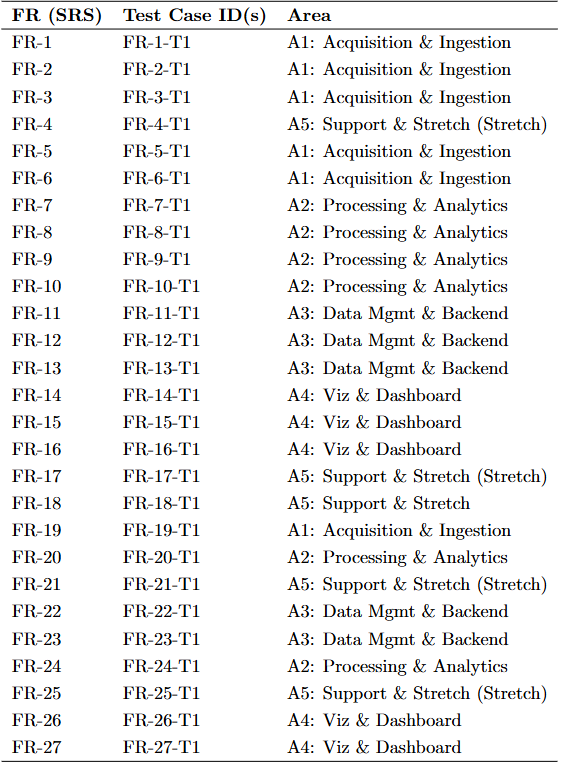
\includegraphics[width=\textwidth]{Images/FR-Tests-Traceability-Matrix.png}
\end{center}

\begin{table}[htbp]
\centering
\caption{Traceability Between NFRs and Test Cases}
\renewcommand{\arraystretch}{1.1}
\small
\begin{tabular}{p{2cm} p{4cm} p{7cm}}
\hline
\textbf{NFR (SRS)} & \textbf{Test Case ID(s)} & \textbf{Area} \\
\hline
NFR-1 & TC-NFR-1-Latency & A1: Data Pipeline \& Ingestion \\
NFR-2 & TC-NFR-2-UpdateHz & A2: Visualization \& Rendering \\
NFR-3 & TC-NFR-3-SyncDrift, TC-NFR-16-Scale10 & A1: Multi-Device Synchronization \\
NFR-4 & TC-NFR-4-JitterLoss & A1: Network Stability \\
NFR-5 & TC-NFR-5-AutoRecover & A1: Data Pipeline Reliability \\
NFR-6 & TC-NFR-6-Uptime & A5: Operational Resilience \\
NFR-7 & TC-NFR-7-Onboarding & A4: Usability \& UI Flow \\
NFR-8 & TC-NFR-8-Contrast & A4: Accessibility \\
NFR-9 & TC-NFR-9-TLSOnly & A3: Security (Transport) \\
NFR-10 & TC-NFR-10-RBAC & A3: Security (Access Control) \\
NFR-11 & TC-NFR-11-AnonStore & A3: Privacy \& Storage \\
NFR-12 & TC-NFR-12-CrossPlat & A5: Portability \\
NFR-13 & TC-NFR-13-Linters & A5: Maintainability (Code Quality) \\
NFR-14 & TC-NFR-14-CI & A5: Maintainability (CI/CD) \\
NFR-15 & TC-NFR-15-Config & A5: Maintainability (Configuration) \\
NFR-16 & TC-NFR-16-Scale10, TC-NFR-3-SyncDrift & A1: Scalability \& Multi-Device Load \\
NFR-17 & TC-NFR-17-TimeACID & A3: Database Integrity \\
NFR-18 & TC-NFR-18-BigSession & A3: Backend Performance \\
NFR-19 & TC-NFR-19-License & A5: Compliance \\
NFR-20 & TC-NFR-20-NonComm & A5: Compliance \\
NFR-21 & TC-NFR-21-UCD & A4: Usability Iteration \\
NFR-22 & TC-NFR-22-Model & A2: Analytics \& Validation \\
NFR-23 & TC-NFR-23-EnvProtocol & A1: Environmental Setup \\
NFR-24 & TC-NFR-24-Consent & A3: Privacy \& Consent Flow \\
NFR-25 & TC-NFR-25-Comfort & A4: User Study Feedback \\
NFR-26 & TC-NFR-26-BackupRestore & A3: Data Backup \& Recovery \\
\hline
\end{tabular}
\end{table}

\section{Unit Test Description}

\wss{This section should not be filled in until after the MIS (detailed design
  document) has been completed.}

\wss{Reference your MIS (detailed design document) and explain your overall
philosophy for test case selection.}  

\wss{To save space and time, it may be an option to provide less detail in this section.  
For the unit tests you can potentially layout your testing strategy here.  That is, you 
can explain how tests will be selected for each module.  For instance, your test building 
approach could be test cases for each access program, including one test for normal behaviour 
and as many tests as needed for edge cases.  Rather than create the details of the input 
and output here, you could point to the unit testing code.  For this to work, you code 
needs to be well-documented, with meaningful names for all of the tests.}

\subsection{Unit Testing Scope}

\wss{What modules are outside of the scope.  If there are modules that are
  developed by someone else, then you would say here if you aren't planning on
  verifying them.  There may also be modules that are part of your software, but
  have a lower priority for verification than others.  If this is the case,
  explain your rationale for the ranking of module importance.}

\subsection{Tests for Functional Requirements}

\wss{Most of the verification will be through automated unit testing.  If
  appropriate specific modules can be verified by a non-testing based
  technique.  That can also be documented in this section.}

\subsubsection{Module 1}

\wss{Include a blurb here to explain why the subsections below cover the module.
  References to the MIS would be good.  You will want tests from a black box
  perspective and from a white box perspective.  Explain to the reader how the
  tests were selected.}

\begin{enumerate}

\item{test-id1\\}

Type: \wss{Functional, Dynamic, Manual, Automatic, Static etc. Most will
  be automatic}
					
Initial State: 
					
Input: 
					
Output: \wss{The expected result for the given inputs}

Test Case Derivation: \wss{Justify the expected value given in the Output field}

How test will be performed: 
					
\item{test-id2\\}

Type: \wss{Functional, Dynamic, Manual, Automatic, Static etc. Most will
  be automatic}
					
Initial State: 
					
Input: 
					
Output: \wss{The expected result for the given inputs}

Test Case Derivation: \wss{Justify the expected value given in the Output field}

How test will be performed: 

\item{...\\}
    
\end{enumerate}

\subsubsection{Module 2}

...

\subsection{Tests for Nonfunctional Requirements}

\wss{If there is a module that needs to be independently assessed for
  performance, those test cases can go here.  In some projects, planning for
  nonfunctional tests of units will not be that relevant.}

\wss{These tests may involve collecting performance data from previously
  mentioned functional tests.}

\subsubsection{Module ?}
		
\begin{enumerate}

\item{test-id1\\}

Type: \wss{Functional, Dynamic, Manual, Automatic, Static etc. Most will
  be automatic}
					
Initial State: 
					
Input/Condition: 
					
Output/Result: 
					
How test will be performed: 
					
\item{test-id2\\}

Type: Functional, Dynamic, Manual, Static etc.
					
Initial State: 
					
Input: 
					
Output: 
					
How test will be performed: 

\end{enumerate}

\subsubsection{Module ?}

...

\subsection{Traceability Between Test Cases and Modules}

\wss{Provide evidence that all of the modules have been considered.}
				
\bibliographystyle{plainnat}

\bibliography{../../refs/References}

\newpage

\section{Appendix}

This is where you can place additional information.

\subsection{Symbolic Parameters}

The definition of the test cases will call for SYMBOLIC\_CONSTANTS.
Their values are defined in this section for easy maintenance.

\subsection{Usability Survey Questions?}

\wss{This is a section that would be appropriate for some projects.}

\newpage{}
\section*{Appendix --- Reflection}

\wss{This section is not required for CAS 741}

The information in this section will be used to evaluate the team members on the
graduate attribute of Lifelong Learning.

The purpose of reflection questions is to give you a chance to assess your own
learning and that of your group as a whole, and to find ways to improve in the
future. Reflection is an important part of the learning process.  Reflection is
also an essential component of a successful software development process.  

Reflections are most interesting and useful when they're honest, even if the
stories they tell are imperfect. You will be marked based on your depth of
thought and analysis, and not based on the content of the reflections
themselves. Thus, for full marks we encourage you to answer openly and honestly
and to avoid simply writing ``what you think the evaluator wants to hear.''

Please answer the following questions.  Some questions can be answered on the
team level, but where appropriate, each team member should write their own
response:


\begin{enumerate}
  \item What went well while writing this deliverable? 
  \begin{itemize}
      \item \textbf{Angela} Writing this deliverable went fine since I focused on mapping the FR tests to requirements. Having the SRS finalized helped make the traceability and test design process straightforward.  
      \item \textbf{Ann} ...
      \item \textbf{Ibrahim} The team benefitted from meeting with the supervisors and research group prior to completing this deliverable, and had a better and more tangible understanding of the project requirements and goals.
      \item \textbf{Manan} ...
      \item \textbf{Stanley} The SRS was settled, so this went quickly. I mapped FR tests to modules and kept the write-up tight to match the template.
    \end{itemize}
  \item What pain points did you experience during this deliverable, and how
    did you resolve them?
  \begin{itemize}
      \item \textbf{Angela} The main challenge was ensuring the test cases aligned correctly with the requirements, especially when some FRs were broad. I resolved this by reviewing our SRS revision and confirming test coverage with the team.
      \item \textbf{Ann} ...
      \item \textbf{Ibrahim} There were some concerns regarding how to format reviews for the documentation, but after meeting with the supervisors, the team was able to work with them to devise a collaborative plan for both the reviews in this deliverable and future documents.
      \item \textbf{Manan} ...
      \item \textbf{Stanley} Hardest part was choosing the right level of detail. I cut jargon and reorganized 3.3–3.6 so they read cleanly.
    \end{itemize}

  \item What knowledge and skills will the team collectively need to acquire to
  successfully complete the verification and validation of your project?
  Examples of possible knowledge and skills include dynamic testing knowledge,
  static testing knowledge, specific tool usage, Valgrind etc.  You should look to
  identify at least one item for each team member.
  \begin{itemize}
      \item \textbf{Angela} I will need to strengthen my understanding of test automation and CI workflows to help verify FR-level functionality efficiently.
      \item \textbf{Ann} ...
      \item \textbf{Ibrahim} It will be helpful to gain a better understanding of the full scope of and the constraints generally applied to testing at this phase of an engineering project.
      \item \textbf{Manan} ...
      \item \textbf{Stanley} I need stronger CI skills to tie PyTest and Jest into one pipeline, and practice writing small, maintainable tests.
    \end{itemize}

  \item For each of the knowledge areas and skills identified in the previous
  question, what are at least two approaches to acquiring the knowledge or
  mastering the skill?  Of the identified approaches, which will each team
  member pursue, and why did they make this choice?
  \begin{itemize}
      \item \textbf{Angela} I plan to review CI documentation for GitHub Actions and explore automated testing frameworks like PyTest as it supports the test workflows we will implement later in the project.
      \item \textbf{Ann} ...
      \item \textbf{Ibrahim} I aim to build on this skill by reading into documentation around engineering documents in general, as well as studying past projects.
      \item \textbf{Manan} ...
      \item \textbf{Stanley} Two approaches: (1) study a minimal GitHub Actions template and adapt it; (2) build tiny test jobs in our repo and iterate. I’m starting with (2).
    \end{itemize}

\end{enumerate}

\end{document}